

%% AP Physics MC Questions Archive
%%----------------------------------------


%% Orbits
%%----------------------------------------
\element{ap}{
\begin{question}{orbits-q01}
    Five planets make circular orbits around a star which is much more massive than any of them.
    The mass and orbital radius of each satellite is given.
    Which satellite has the longest period?
    \begin{choices}
        \wrongchoice{Mass: $M$; Radius: $R$}
        \wrongchoice{Mass: $M$; Radius: $R$}
        \wrongchoice{Mass: $M$; Radius: $R$}
        \wrongchoice{Mass: $2M$; Radius: $R$}
      \correctchoice{Mass: $M$; Radius: $2R$}
    \end{choices}
\end{question}
}

\element{ap}{
\begin{question}{orbits-q02}
    A satellite is orbiting around the Earth at a radius of $2R$ from its center.
    What is the magnitude of the velocity it is traveling at?
    \begin{multicols}{3}
    \begin{choices}
      \correctchoice{$\sqrt{\dfrac{GM}{2R}}$}
        \wrongchoice{$\dfrac{GM}{2R}$}
        \wrongchoice{$\dfrac{2GM}{R}$}
        \wrongchoice{\SI{9.8}{\meter\per\second}}
        \wrongchoice{$\dfrac{G}{R}$}
    \end{choices}
    \end{multicols}
\end{question}
}

\element{ap}{
\begin{question}{orbits-q03}
    The Earth exerts the necessary centripetal force on an orbiting satellite to keep it moving in a circle at constant speed.
    Which of the following statements best explains why the speed of the satellite does not change even though there is a net force exerted on it?
    \begin{choices}
        \wrongchoice{The satellite is in dynamic equilibrium.}
        \wrongchoice{The acceleration on the satellite is zero.}
        \wrongchoice{The centripetal force is in the direction of the velocity of the satellite.}
        \wrongchoice{The centripetal force is equivalent to the reaction force caused from the satellite.}
      \correctchoice{The centripetal force is perpendicular to the velocity of the satellite.}
    \end{choices}
\end{question}
}

\element{ap}{
\begin{question}{orbits-q04}
    A satellite in orbit around the Earth has a period of one hour.
    An identical satellite is placed in an orbit having a radius which is nine times larger than the first satellite.
    What is the period of the second satellite?
    \begin{multicols}{3}
    \begin{choices}
        \wrongchoice{\SI{0.004}{\hour}}
        \wrongchoice{\SI{1/3}{\hour}}
        \wrongchoice{\SI{3}{\hour}}
        \wrongchoice{\SI{9}{\hour}}
      \correctchoice{\SI{27}{\hour}}
    \end{choices}
    \end{multicols}
\end{question}
}

\element{ap}{
\begin{question}{orbits-q05}
    A satellite orbits the Earth in at a distance of 1 Earth radius from the surface.
    Its velocity is $v$.
    If the satellite moves and enters a new orbit at 3 Earth radii from the Earth's surface,
        its new velocity will be:
    \begin{multicols}{3}
    \begin{choices}
        \wrongchoice{$\dfrac{v}{2}$}
        \wrongchoice{$v\sqrt{3}$}
        \wrongchoice{$v\sqrt{2}$}
        \wrongchoice{$\dfrac{v}{\sqrt{3}}$}
      \correctchoice{$\dfrac{v}{\sqrt{2}}$}
    \end{choices}
    \end{multicols}
\end{question}
}

\element{ap}{
\begin{question}{orbits-q06}
    If the radius of a satellite's orbit is doubled,
        it's kinetic energy will:
    \begin{choices}
        \wrongchoice{be doubled.}
      \correctchoice{be halved.}
        \wrongchoice{decrease by a factor of 4.}
        \wrongchoice{increase by a factor of 4.}
        \wrongchoice{remain the same.}
    \end{choices}
\end{question}
}

\element{ap}{
\begin{question}{orbits-q07}
    A moon orbits a planet in a circular orbit of radius $R$.
    If the mass of the planet is $M$,
        what is the period of the moon's revolution?
    \begin{multicols}{3}
    \begin{choices}
        \wrongchoice{$\pi\sqrt{\dfrac{R^3}{GM}}$}
        \wrongchoice{$\pi\sqrt{\dfrac{R^2}{GM}}$}
        \wrongchoice{$2\sqrt{\dfrac{R^2}{GM}}$}
      \correctchoice{$2\pi\sqrt{\dfrac{R^3}{GM}}$}
        \wrongchoice{$\dfrac{\pi}{2}\sqrt{\dfrac{R^3}{GM}}$}
    \end{choices}
    \end{multicols}
\end{question}
}

\element{ap}{
\begin{question}{orbits-q08}
    %Base your answers to questions 8 and 9 on the following.
    An astronomical unit (AU) is defined as the mean distance at which the Earth orbits the Sun.
    %% start question
    If the planet $P$ orbits at a mean distance of 6 AU,
        a year on $P$ is most nearly:
    \begin{multicols}{2}
    \begin{choices}
        \wrongchoice{3 Earth years}
        \wrongchoice{6 Earth years}
      \correctchoice{15 Earth years}
        \wrongchoice{39 Earth years}
        \wrongchoice{216 Earth years}
    \end{choices}
    \end{multicols}
\end{question}
}

\element{ap}{
\begin{question}{orbits-q09}
    %Base your answers to questions 8 and 9 on the following.
    An astronomical unit (AU) is defined as the mean distance at which the Earth orbits the Sun.
    %% start question
    The planet Krypton orbits a star 2 times more massive than the Sun.
    It takes 27 Earth years to circle this star.
    The radius of Krypton's orbit is most nearly:
    \begin{multicols}{3}
    \begin{choices}
        \wrongchoice{5 AU}
      \correctchoice{9 AU}
        \wrongchoice{18 AU}
        \wrongchoice{27 AU}
        \wrongchoice{44 AU}
    \end{choices}
    \end{multicols}
\end{question}
}

\element{ap}{
\begin{questionmult}{orbits-q10}
    A satellite moves in a circular orbit around a planet at a constant speed.
    Which of the following must be true?
    \begin{choices}
      \correctchoice{The net force on the satellite is always radially inward.}
      \correctchoice{The net work done on the satellite in the interval of half an orbit is zero.}
      \correctchoice{The angular momentum of the satellite is constant.}
    \end{choices}
\end{questionmult}
}

\element{ap}{
\begin{question}{orbits-q11}
    The Moon, mass $m$, orbits the Earth, mass $M$,
        in a circular orbit with radius $r$.
    What is the kinetic energy of the Moon in its orbit?
    \begin{multicols}{3}
    \begin{choices}
        \wrongchoice{$\dfrac{GMm}{2r}$}
        \wrongchoice{$\dfrac{GMm}{4r}$}
      \correctchoice{$\dfrac{GMm}{r}$}
        \wrongchoice{$\dfrac{GMm}{r^2}$}
        \wrongchoice{$\dfrac{GMm}{4r^2}$}
    \end{choices}
    \end{multicols}
\end{question}
}

\newcommand{\apOrbitsQTwelve}{
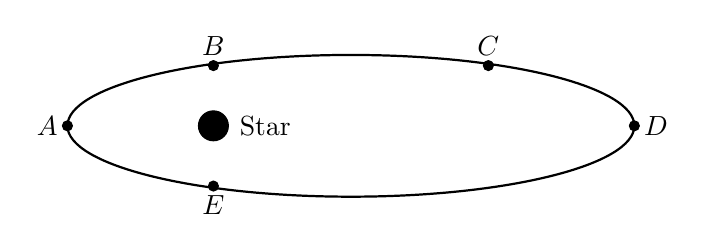
\begin{tikzpicture}[scale=0.9]
    %% orbit and center
    \draw[thick] (0,0) circle (4cm and 1cm);
    \draw[fill] (-1.94,0) circle (6pt) node[anchor=west,xshift=6pt] {Star};
    %% options are lower case
    \draw[fill] (-4,0) circle (2pt) node[anchor=east] {$A$};
    \draw[fill] (-1.94,0.85) circle (2pt) node[anchor=south] {$B$};
    \draw[fill] (+1.94,0.85) circle (2pt) node[anchor=south] {$C$};
    \draw[fill] (+4,0) circle (2pt) node[anchor=west] {$D$};
    \draw[fill] (-1.94,-0.85) circle (2pt) node[anchor=north] {$E$};
\end{tikzpicture}
}

\element{ap}{
\begin{question}{orbits-q12}
    %Base your answers to questions 12 and 13 on the picture below,
    The picture below represents a planet that moves in an elliptical orbit with a star as one focus as shown below.
    \begin{center}
        \apOrbitsQTwelve
    \end{center}
    At which point does the planet have the greatest potential energy?
    \begin{multicols}{5}
    \begin{choices}[o]
        \wrongchoice{$A$}
        \wrongchoice{$B$}
        \wrongchoice{$C$}
      \correctchoice{$D$}
        \wrongchoice{$E$}
    \end{choices}
    \end{multicols}
\end{question}
}

\element{ap}{
\begin{question}{orbits-q13}
    %Base your answers to questions 12 and 13 on the picture below,
    The picture below represents a planet that moves in an elliptical orbit with a star as one focus as shown below.
    \begin{center}
        \apOrbitsQTwelve
    \end{center}
    At which two points does the planet have the same velocity?
    \begin{multicols}{3}
    \begin{choices}
        \wrongchoice{$A$ and $E$}
        \wrongchoice{$A$ and $D$}
        \wrongchoice{$B$ and $C$}
      \correctchoice{$B$ and $E$}
        \wrongchoice{$C$ and $D$}
    \end{choices}
    \end{multicols}
\end{question}
}

\element{ap}{
\begin{question}{orbits-q14}
    The square of the period of an orbit is proportional to the cube of the semimajor axis of the orbit.
    This statement is best known as:
    \begin{choices}
        \wrongchoice{Kepler's First Law}
        \wrongchoice{Kepler's Second Law}
      \correctchoice{Kepler's Third Law}
        \wrongchoice{Conservation of angular momentum}
        \wrongchoice{None of the above}
    \end{choices}
\end{question}
}

\element{ap}{
\begin{question}{orbits-q15}
    Planets sweep out equal areas in equal times.
    This statement is best known as:
    \begin{choices}
        \wrongchoice{Kepler's First Law}
      \correctchoice{Kepler's Second Law}
        \wrongchoice{Kepler's Third Law}
        \wrongchoice{Conservation of angular momentum}
        \wrongchoice{None of the provided}
    \end{choices}
\end{question}
}

\element{ap}{
\begin{question}{orbits-q16}
    The planets orbit in elliptical paths with the sun at one focus of the ellipse.
    This statement is best known as:
    \begin{choices}
      \correctchoice{Kepler's First Law}
        \wrongchoice{Kepler's Second Law}
        \wrongchoice{Kepler's Third Law}
        \wrongchoice{Conservation of angular momentum}
        \wrongchoice{None of the provided}
    \end{choices}
\end{question}
}

\element{ap}{
\begin{question}{orbits-q17}
    What is the total energy of a satellite of mass $m$ that orbits a planet of mass $M$ in an elliptical orbit with semi-major axis $a$?
    \begin{multicols}{3}
    \begin{choices}
      \correctchoice{$\dfrac{-GMm}{2a}$}
        \wrongchoice{$\dfrac{-GMm}{a}$}
        \wrongchoice{$\dfrac{GMm}{4a}$}
        \wrongchoice{$\dfrac{GMm}{2a}$}
        \wrongchoice{$\dfrac{GMm}{a}$}
    \end{choices}
    \end{multicols}
\end{question}
}

\element{ap}{
\begin{question}{orbits-q18}
    A planet orbits around a star which is not at the center of its orbit.
    The shape of the orbit is most likely:
    \begin{multicols}{2}
    \begin{choices}
        \wrongchoice{circular}
        \wrongchoice{parabolic}
      \correctchoice{elliptical}
        \wrongchoice{hyperbolic}
        \wrongchoice{spherical}
    \end{choices}
    \end{multicols}
\end{question}
}


\endinput


